\section{Speckle pattern} \label{Speckle pattern} 
Speckle patterns er betegnelsen for et billede eller område med prikker, der anvendes til måling af deformationer og tøjninger i materialer ved brug af DIC \parencite{Dong2017ACorrelation}. Prikkerne i et speckle pattern er ikke foruddefineret til at have én bestemt størrelse, form, kontrast, densitet og fordeling. Disse parametre afhænger af størrelsen på emnet der undersøges, kameraets opløsning samt påføringsmetoden. Eksempler på forskellige speckle patterns kan ses i figur \ref{fig:speckle pattern}.\\

\begin{figure}[H]
    \centering
    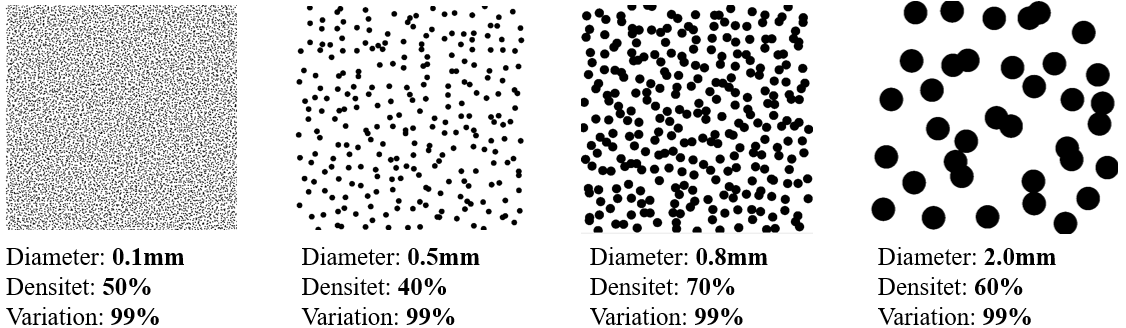
\includegraphics[width=\linewidth]{Sections/2 Problemanalyse/Media/speckle pattern forskellige.png}
    \caption{Eksempler på computergenereret speckle patterns med forskellig densitet og prikstørrelse. Speckle pattern er genereret med software fra Correlated Solutions (\cite{CorrelatedSolutions2025SpeckleInc.})}
    \label{fig:speckle pattern}
\end{figure} \plainbreak{-0.5}

Præcisionen af DIC afhænger blandt andet af det anvendte speckle patterns kvalitet, der kan vurderes ved brug af softwareprogrammer. Programmerne benytter forskellige metoder til kvalitetsvurdering, der vurderer parametre som størrelse, form og fordeling af prikkerne. 